\chapter{Methods and experiments}
\thispagestyle{pagestyle}

% Figures are generated under repository ``outputs/`` (relative to this file: two levels up to repo root).
\graphicspath{{../../outputs/}}

\section{Methods}

\subsection{Image representation and FRQI encoding}
Grayscale test images are square arrays of side length $N \in \{4,8,16\}$ (uint8 intensities). The \emph{flexible representation of quantum images} (FRQI) encodes each pixel amplitude into one qubit angle and uses a position register of $m = 2\log_2 N$ qubits so that $N_{\mathrm{pix}} = N^2 = 2^m$ addresses cover all pixels. The implementation follows \texttt{src/frqi.py}: angles $\theta_p = (\pi/2)\cdot (\mathrm{intensity}_p/255)$ align with Qiskit's \texttt{Ry} convention, and the computational-basis index orders the position register with the \textbf{color qubit as the least significant bit} (same register ordering as the structural circuits in \texttt{src/improved.py}).

\subsection{QHED baseline and classical Sobel}
The quantum-inspired Hadamard edge detector (QHED) baseline applies a 2D fast Walsh--Hadamard transform, uses the magnitude spectrum as a contrast proxy, inverts back to the spatial domain, and finally applies a classical $3\times 3$ Sobel magnitude (\texttt{src/qhed.py}). Classical Sobel on the original image serves as a lightweight reference edge map for comparisons.

\subsection{Structural FRQI preparation: naive vs v-chain MCX}
The thesis compares two gate-level preparations of the same ideal FRQI state:
\begin{itemize}
  \item \textbf{Naive decomposition:} per-pixel address compare, multi-controlled $X$ into a workspace qubit using Qiskit's \texttt{MCXGate(..., mode="noancilla")}, controlled \texttt{cry($2\theta_p$)} on the color qubit, then uncompute. This follows the textbook worst-case scaling for multi-controlled rotations without dedicated ancilla (exponential-in-$m$ cost per slice in the worst case).
  \item \textbf{Improved (ancilla-assisted) path:} the same logical pattern with \texttt{mode="v-chain"}, reusing up to $m-2$ dirty ancillas so each multi-controlled $X$ uses $O(m)$ CX rather than $O(2^m)$ in the no-ancilla mode. Full naive transpilation is only practical for $4\times 4$ in this repository; for $8\times 8$ and $16\times 16$ the CSV reports a \texttt{struct\_naive\_slice\_scaled} row obtained by transpiling one representative slice and multiplying depth/CX by $N_{\mathrm{pix}}$ (linear MCX scaling estimate; see \texttt{thesis/design/resource\_and\_complexity.md}).
\end{itemize}

\subsection{Noise model and image metrics}
Noisy experiments use Qiskit Aer \texttt{density\_matrix} simulation with depolarizing errors on one- and two-qubit gates (\texttt{src/noise\_models.py}). Optional thermal relaxation and readout error hooks exist for API compatibility; unless a shot-based demo is enabled, readout noise does not alter the stored density matrix. After simulation, the state is partially traced to the FRQI data register (color plus position), converted to a pixel reconstruction, and compared to the clean image using peak signal-to-noise ratio (PSNR), structural similarity (SSIM via scikit-image), and state fidelity against the ideal FRQI statevector.

\subsection{Readout mitigation (concept)}
For shot-based readout on real hardware, a practical mitigation path is an empirical $2\times 2$ confusion matrix for the color qubit, its (regularized) inversion, and application to measured outcome probabilities (\texttt{thesis/design/readout\_mitigation.md}; prototype helper \texttt{run\_readout\_mitigation\_slice\_demo} in the codebase).

\section{Experimental setup}

\subsection{Data and software}
Datasets live in \texttt{data/test\_images/} as \texttt{test\_4x4.npy}, \texttt{test\_8x8.npy}, and \texttt{test\_16x16.npy}. The experiments in this chapter were run with the Python stack pinned in \texttt{requirements.txt} (Qiskit~1.x, Qiskit Aer, NumPy, SciPy, Matplotlib, pandas, scikit-image). All circuits in this submission use \textbf{simulators only}; hardware runs, if added later, should record backend name, basis gates, and layout.

\subsection{Reproducible commands}
\begin{itemize}
  \item \textbf{Demo (FRQI + QHED figures):} \texttt{python scripts/demo\_frqi\_qhed\_sobel.py}
  \item \textbf{Structural resources (CSV + CX/depth plots):} \texttt{python scripts/frqi\_structural\_resources.py} \\
        Writes \texttt{outputs/frqi\_structural\_metrics.csv}, \texttt{outputs/fig\_cx\_vs\_image\_size.png}, and \texttt{outputs/fig\_depth\_vs\_image\_size.png}. Use \texttt{--plot-only} to redraw from an existing CSV.
  \item \textbf{Noisy FRQI sweep:} \texttt{python scripts/noisy\_frqi\_sweep.py} \\
        Default images \texttt{test\_4x4,test\_8x8,test\_16x16}. Density-matrix RAM scales as $4^{n_q}$ in the worst case; the script skips $16\times 16$ v-chain ($16$ qubits) unless \texttt{--allow-heavy-dm} is passed---use a coarser \texttt{--scales} grid if enabling that run. Outputs: \texttt{outputs/noisy\_frqi\_metrics.csv} and per-image curve PNGs.
  \item \textbf{Optional edge ablation (noisy recon $\rightarrow$ QHED vs Sobel):} \texttt{python scripts/noisy\_recon\_qhed\_edge\_metrics.py}
\end{itemize}

\section{Results and figures}

\subsection{Transpiled structural cost vs image size}
\cref{fig:cx-vs-n} summarizes transpiled two-qubit (\texttt{cx}) counts after decomposition to \texttt{cx,rz,sx} at optimization level~3. The v-chain full preparation grows far more slowly than the scaled naive estimate derived from one transpiled \texttt{noancilla} slice.

\begin{figure}[htbp]
\centering
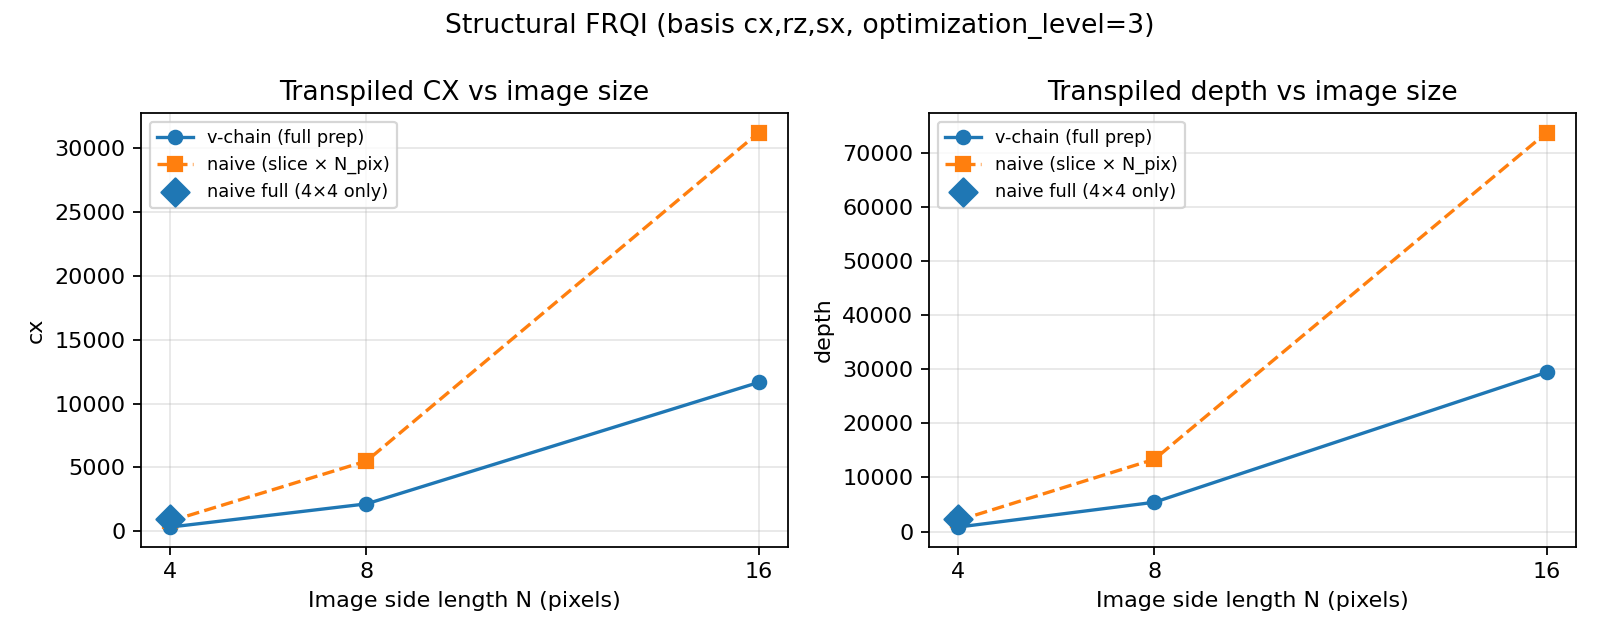
\includegraphics[width=0.95\textwidth]{fig_cx_vs_image_size.png}
\caption{Transpiled CX and depth vs linear image size $N$ for structural FRQI: v-chain full preparation, naive linear extrapolation from one slice (\texttt{struct\_naive\_slice\_scaled}), and the full naive $4\times 4$ point where available.}
\label{fig:cx-vs-n}
\end{figure}

\subsection{Robustness of noisy FRQI reconstruction}
\cref{fig:noisy-4} shows fidelity, PSNR, and SSIM as depolarizing strength scales for each test resolution. For $16\times 16$, the default simulator configuration includes the naive layout (10~qubits) but omits v-chain rows when the qubit cap is exceeded; see the Experimental setup section.

\begin{figure}[htbp]
\centering
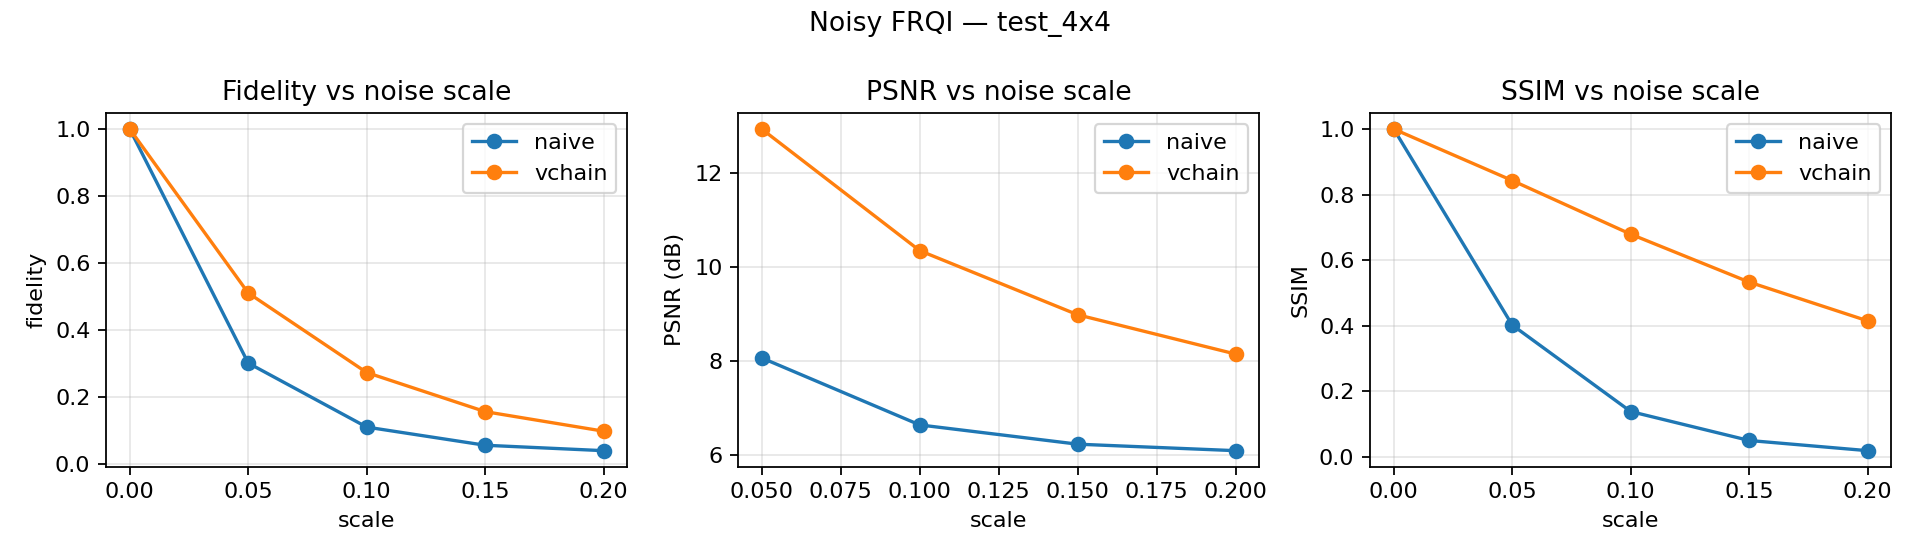
\includegraphics[width=0.95\textwidth]{noisy_frqi_test_4x4_curves.png}
\caption{Noisy FRQI preparation on \texttt{test\_4x4}: fidelity, PSNR, and SSIM vs noise scale for naive vs v-chain circuits.}
\label{fig:noisy-4}
\end{figure}

\begin{figure}[htbp]
\centering
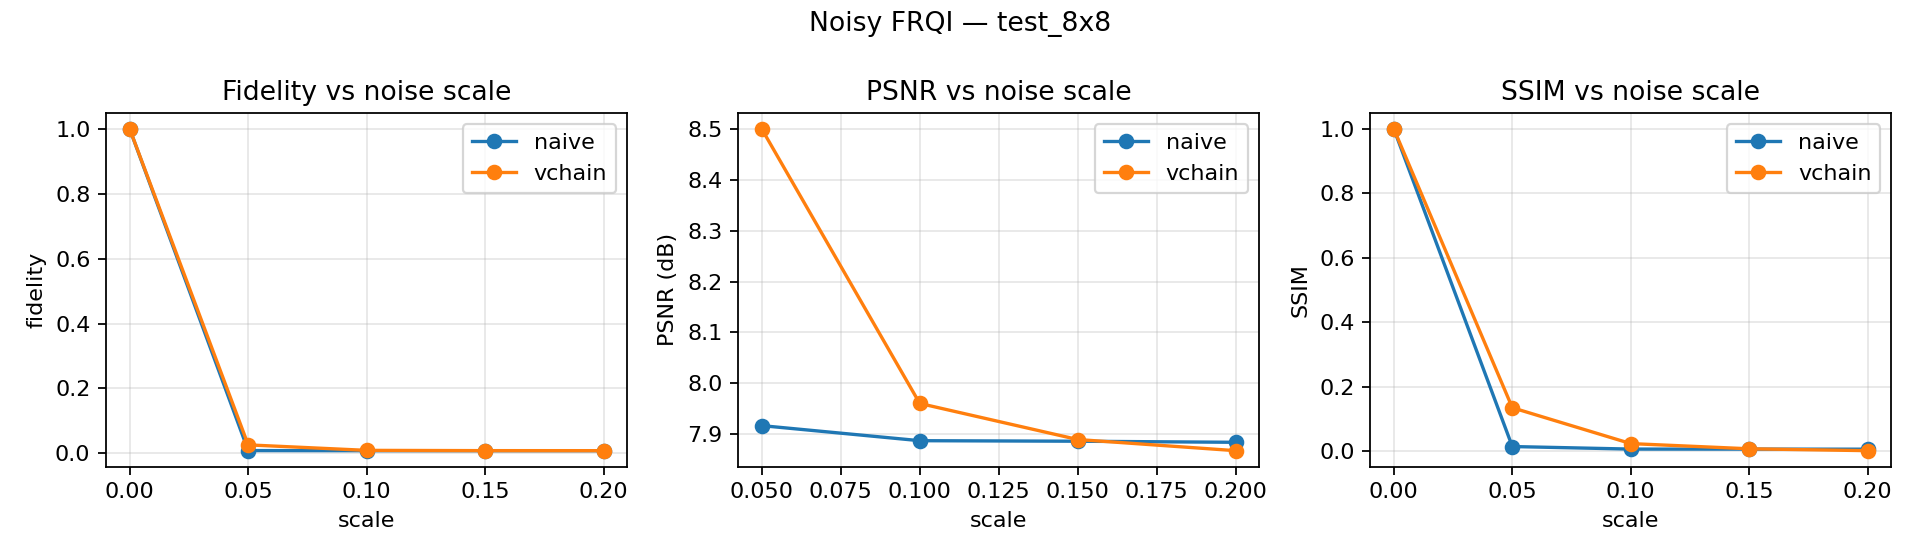
\includegraphics[width=0.95\textwidth]{noisy_frqi_test_8x8_curves.png}
\caption{Same metrics for \texttt{test\_8x8}.}
\label{fig:noisy-8}
\end{figure}

\begin{figure}[htbp]
\centering
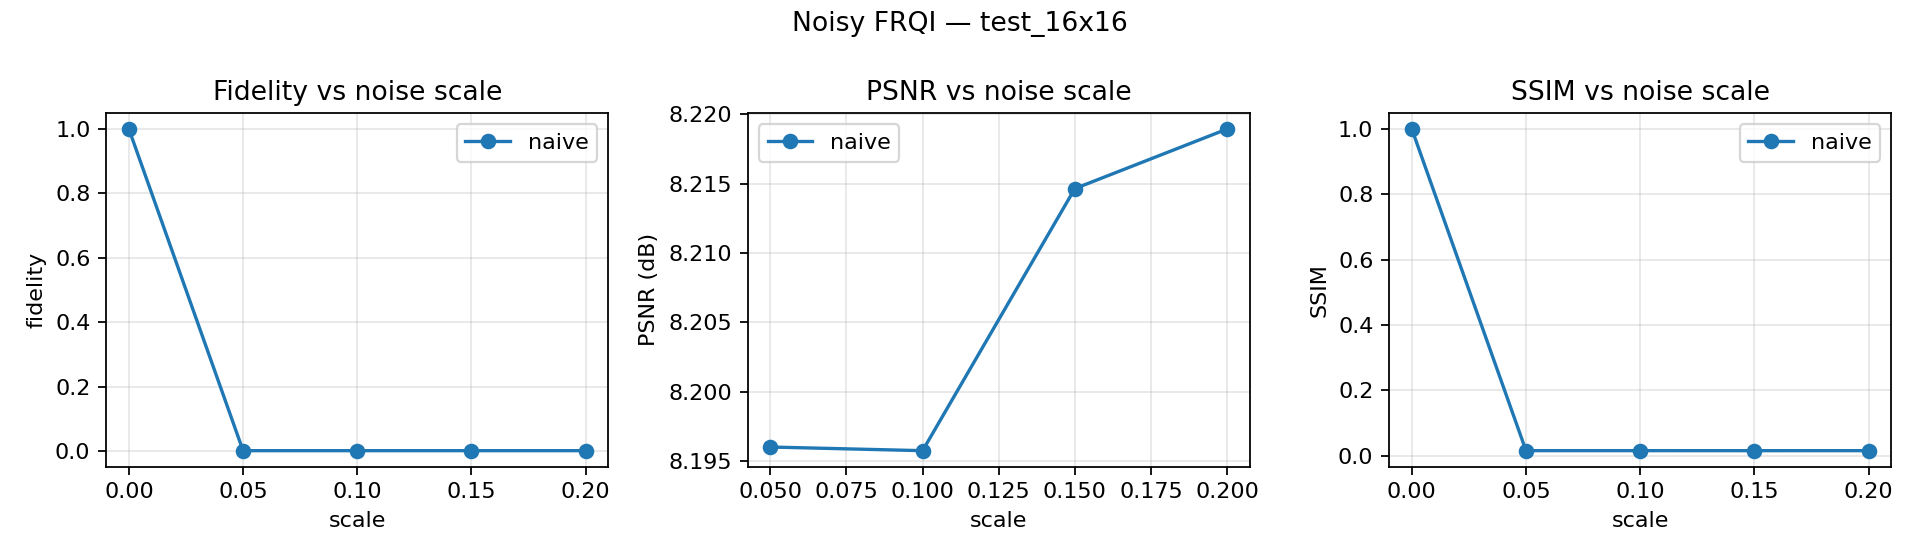
\includegraphics[width=0.95\textwidth]{noisy_frqi_test_16x16_curves.png}
\caption{Same metrics for \texttt{test\_16x16} (default run: naive only if v-chain is skipped for RAM).}
\label{fig:noisy-16}
\end{figure}

\subsection{Optional: edge maps from noisy reconstructions}
When \texttt{scripts/noisy\_recon\_qhed\_edge\_metrics.py} is run, compare the resulting \texttt{outputs/noisy\_recon\_qhed\_edges\_*.png} files; they report PSNR/SSIM between the QHED edge map applied to the noisy reconstruction and the Sobel edge map of the clean original.
